\section{Introduction}

% In the process of musical composition, composers tend to follow a strict set of theories and guidelines to maintain the aesthetic quality of the music they create \cite{rothgeb1975strict,collins2005synthesis,kikuchi2016music}. The process is usually not standardized and can be customized depending on the task of the composer. As such, one composer's approach might not work effectively for another \cite{cheng2016approaching,collins2016act}. To address this, we present a tool that will assist in the process rather than force composers to adapt to an unnatural approach. We intend to minimize cognitive load in every stage of the composition process. But generally, composers undergo a series of activities that allow them to draft their musical products, regardless of order or sequence \cite{bennett1976process,graf2013beethoven}. These are (1) ideation, (2) sketching, and (3) revision. We developed a product that enables composers to undergo these stages, while ensuring a user-centric approach in the process. \\

% Members of the DHH community are unable to fully hear music through conventional means, which may lead to various emotional and social challenges, including expressing emotions \cite{Walker:2013}, making meaningful social connections, and even recognizing their own environment and culture \cite{Ribiero:2017}. One of the solutions developed for this problem is the usage of cochlear implants, which are composed of processors outside of the skin, and an implant placed inside the cochlea. However, cochlear implants do present drawbacks, and may not be sufficient as a stand-alone solution to the problems experienced by the DHH community due to technical limitations \cite{Gfeller:2012, Drennan:2015,Moran:2016}. There have been two main approaches in augmenting the DHH musical experience. The first is through haptic means, to which there have already been several approaches done by previous research \cite{Jack:2015, Nanayakkara:2009:EME, Petry:2016}. The second is through visual means, such as that done by \cite{Jain:2015}, and is the approach taken by this research. This research attempts to make these four (4) contributions: (1) the design of an interaction that seeks to improve how the DHH experience music, (2) the exploration of the use of a movie roll visualization scheme which allows for more creative visuals towards augmenting these experiences \cite{Nanayakkara:2007}, (3) the development of a framework to process and understand music samples towards generating the appropriate visualizations and (4) the evaluation on whether these ultimately augment the music experiences of the DHH.
% A framework is introduced following the approach done by \cite{deja2019myosl}, and current work is presented along with the proposed next steps. 

Music, is an effective learning companion for children. This makes music play an important role in their education \cite{levinowitz1999importance}. It has also been said that music is part of a child’s playful nature that helps contribute to their overall development \cite{mcpherson2015child}. This playful nature could involve spontaneous singing, sound exploration, and dance. Yet the difficulty in teaching a child to learn music is on how to make it enjoyable for them, as the learning comes from them exploring various instruments at an early age \cite{ghazali2005minds}. There are many different approaches that help in learning. One common way is children attending traditional schools as they use the instructional approach of learning where there is a teacher guiding them throughout the process. Another approach which is mostly unconventional in schools is the use of mnemonics where relatable associations are used to remember complex ideas \cite{putnam2015mnemonics}. 

Next is the use of a sandbox approach where the child can playfully learn using a virtual sandbox environment on their own. Here, they discover by themselves the ideas by exploring and playing around the sandbox environment. A sandbox environment is where users can play without the fear of destroying something \cite{burton2016music}.  We want to discover whether these technologies such as implementing a virtual sandbox environment can enable children to play, create and explore music. The development of Scratch, a visual programming language that makes use of blocks as instructions, implemented a sandbox approach to a programming tutorial software \cite{maloney2010scratch}. This application made it possible for children to play around, explore, and learn at their own pace. By using the sandbox approach, Scratch was able to teach a difficult and complex task to a child. Other works of the same approach are now outdated like the sandbox application Otomushi \cite{andre2010otomushi}. It proposed a unique sandbox environment for sound exploration by mixing virtual creatures and scratching techniques. While there have been many works that help children only few have used their playful nature as they interact with music. These works have shown that children require different methods for teaching compared to adults due to their different needs like having short attention spans, and requiring many repetitions when being taught music. Our work helps in designing a usable mobile musical learning tool for children that helps in creating a child friendly interface for children to learn a hard concept like music. By using different visual design principles and heuristics we can create an interface that can help us in identifying and modelling the human factors and behaviours that children exhibit when given the task of learning how to compose music with a mobile musical tool. We did a study that composed of interviews and user tests with the target participants. We then developed prototypes based on the different findings which were iteratively tested to the users. In this study we: (1) Understand the process how children learn music, through the help of music teachers, (2) to design an interaction that helps the children in creating easier gestures for interaction, (3) develop an application which makes use of a sandbox environment that will help children in learning music, and lastly (4) evaluate whether these ultimately help in improving the music learning of the children and identify the human factors that they exhibit.
\section{Related Work}
This  chapter  discusses  the  features,  capabilities,  and  limitations  of  existing  research, algorithms, or software that are related/similar to the thesis. This will help us identify features that we can use, and limitations that we can improve.
\subsection{Playful Interactions for Children}
Five commercially available applications for preschool children was analyzed \cite{gray2018designing}. It was discussed that some factors in these applications may lead to children liking or disliking the application. It was also said that the importance of characters, support for competence, interaction complexities, and the understanding of buttons and menus. Different game characters with different personalities may increase the chances of a child liking a character which would contribute to the game's enjoyment. Support for competence involves a child getting in-game rewards for doing good in the game. Interaction complexities described that confusing tutorials such as one where actual game play cannot be differentiated from a tutorial makes it confusing for the child.

Play has a different definition for children as it does for adults \cite{scheepmaker2018things}. The children are in control meaning they started playing because they want to. Playing for them includes things that they do not need to finish or seek approval. An important aspect of play is called appropriation. Playful appropriation is a transformation of situations or elements into fun experiences. An example seen in the paper involved an animal like robot designed to bring out certain behaviors in children. The different children had different abilities and experiences therefor leading to them having different ways to appropriate the robot into their own versions of play. This leads to the idea of designing applications for appropriation. These designs are defined to be ambiguous,in need of a user who will complete them and break away from a usual designer-centered thinking where the system makes it clear how the system should be interacted with. 
In general, it is a mindset where something is approached without seriousness or a clear goal \cite{li2018understanding}. Playfulness may help in making products go beyond their initial level of entertainment. This idea discusses interaction for play is a three stage model. The three stages are invitation, exploration and immersion \cite{crowell2018role}. Invitation is the state where the system should invite the user to engage with it. Exploration is when the user is trying out different possibilities with the system. Finally immersion happens when the user has explored enough with the system and is creating different things that applies everything learned in the exploration stage.

Scratch is one example of an application that implemented a sandbox approach. It allows users to drag and drop blocks to control 2D graphical objects moving on the background. One of the most important feature of Scratch is that it is always live, meaning it requires no compilation step or run mode. Users can also add blocks while a script is running. This lets users be engaged with their projects and always be able to tinker with the blocks \cite{maloney2010scratch}. In the study of \citeA{ouahbi2015learning}, high school students were able grasp programming concepts, and syntax was also not an issue for them. In addition to this, Scratch allows easy visualization of how the algorithm is looks like, and in effect increasing a user’s motivation to learn programming \cite{erol2017effects}. By implementing these features, Scratch is able to provide users a sandbox environment that enables them to learn programming. 

OtoMushi, derived from its Japanese meaning where \textit{oto} means sound and \textit{mushi} means insect, is a platform for interacting with sound samples which is represented by insects developed by Andre (2010). Its sandbox environment allows a controlled canvass where users can mix virtual creatures applying scratching techniques to explore sound \cite{andre2010otomushi}. It allows users to record sound when they speak. A tangible sandbox environment surface called smartskin by \cite{rekimoto2002smartskin} lacked responsiveness and that the resolution of the graphics were bad. In later iterations, OtoMushi was implemented on the iPad. By implementing it this way, children can play with the tool as if it was a virtual sandbox environment. With this, a child's playfulness can be exploited by allowing them to play with the tool as much as they want.

\subsection{Music Teaching Apps for Children}
There are several music applications that are not sandbox in approach but still provide virtual collaborative environments for expression and composition. MOGCLASS is a multimodal collaborative music environment that enhances students’ musical experience and improves teacher’s management of the classroom \cite{zhou2011mogclass}. This application features an interface for the teacher and a separate interface for the students. The teacher’s interface has features that allow the teacher to manage the class better, while the student’s interface has features that mimic instruments this supports a music technique called scaffolding.
MOGCLASS simulates 3 instruments for the students and can be seen in 3 different student interfaces. The first instrument is called a hitter and it stimulates a drum. It uses an accelerometer in which makes the device detects handshakes and makes a sound proportional to the level of shaking. The second instrument is called a tapper which stimulates a piano. The location of the bar shows which note to be played and the size of the bar shows how long the note should be played. The last instrument is the slider and it stimulates a violin. The vertical position of the finger plays different notes on the slider.

The development of musical tools have migrated to mobile environments as well. SAMI is a music learning application for children using tablet-computers. For it to be able to teach music, it has 4 games that are designed to facilitate learning and encourage children's thinking and creativity \cite{paule2017music}. The first game aims to educate the children by using the ears to identify several sounds. In short, the first game is a memory game using notes. The game plays a note and the task of the user is to tap SAMI with a similar noise representing that note. Each SAMI has a color at first to determine the note. The second game is a memory game with order of the notes wherein the children have to tap on SAMIs in the correct order. This aims to teach notes as if they were part of a major chord. The third game is a reactive tapping game and aims to teach fine motor skills required to play instruments. There are 3 rows and each location of SAMI places a different note. SAMIs appear and the child needs to tap on SAMI before they disappear. SAMIs on the top row play higher pitched notes when tapped. The last game is a composing game which combines all the previous games and has the child try to compose with SAMIs by having arrange SAMI’s in different heights and at a certain arrangement. These games may serve as an inspiration on how some features or parts of FireflyX may be able to be implemented.

Just as SAMI teaches with its games, an application by \cite{elahi2017xylotism} also teaches with instructions. This application features a bot named Nima that gives instructions. The instructions given by Nima follow a step by step process. The initial stages would be instructions to get the user to understand notes. These instructions include commands for the user to do something or questions to ask the user. The later stages would involve trying to make the user replicate rhythms. Based on the user's actions, Nima also gives some feedback to help guide the user. When the user is doing well, Nima can respond by doing dances and saying things like that's great, bravo, etc. If the user makes a mistake, Nima says things like pay attention or try again. Aside from these responses, there are also emojis showing happy faces or sad faces depending on the user's actions as well. From this application, FireflyX may be able to use the instructions and feedback system given by Nima. The instruction system may help guide the children on the usage of FireflyX. The feedback system may encourage the children with their usage of FireflyX.

Multimedia Technology has been widely used in the education of students especially in the field of teaching music \cite{tong2016design}. Examples of these technologies include applications such as Musilla Musical School \cite{educationalappstore2017}, which is an application designed to teach the principles of music to children. Another is Sesame Street Makes Music \cite{educationalappstore2015}, which is an application designed to help children explore instruments, tempo, and musical creativity. However these applications pose further opportunities for learning such as the limitations in accurate representations.

\section{Methodology}
The methodology for this study can be divided into 3 phases can seen in Figure \ref{fig:research_framework}. The first phase (Phase 1), dealt with understanding the students and identify their needs with the help of their music teacher. Using the data gathered from the interview with the teachers, the next phase (Phase 2) involved the designing of the interaction to solve the needs of the students. The last phase (Phase 3) is a constant process of testing and developing on the proposed solution based on the feedback gathered in each tests with the user.

\begin{figure}[H]
    \centering
    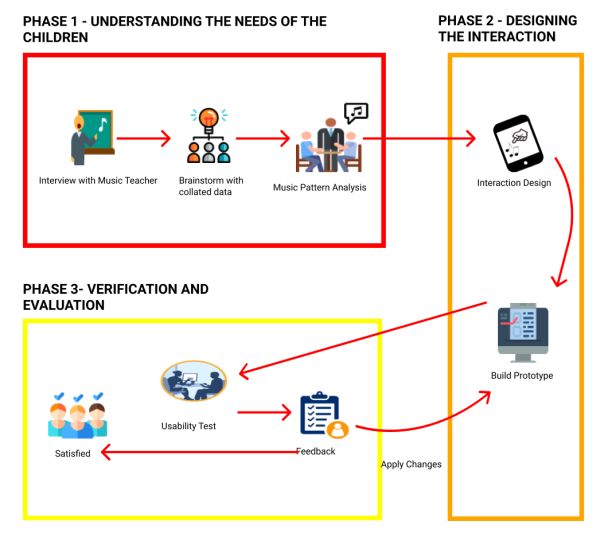
\includegraphics[width=8.5cm,height=7.5cm]{NewFigures/ResFramework.png}
    \caption{Overview of the different phases of the research methodology}
    \label{fig:research_framework}
\end{figure}

% PHASE 1

\subsection{Formative Study}
We recruited music experts using snowball sampling. The experts we consulted were generally categorized as music teachers and had been teaching music for at least 5 years. We interviewed these experts in order for us to understand the different processes on how children are taught music. This interview was also done to expand our knowledge on music and identify the approaches these teachers would do in teaching children. The notes taken during the interview was used for discussion within the group to collate and brainstorm. Questions were designed to be open-ended so that the interviewees included more detail to answering the question and also for the researchers to extract more information from the interviewee. Below are some questions asked in the interviews:

\begin{itemize}
    \item How long have you been teaching music?
    \item How do you start your sessions with children?
    \item Do you have special techniques when teaching children?
    \item Do you use the same techniques with all the children?
    \item What difficulties do you encounter when you teach children?
    \item Do you keep in contact with the student outside the classroom?
    \item What role do the parents have in the learning journey of the child?
\end{itemize}

After the interviews, we analyzed and processed the data acquired. Based on the problem statement, we then developed ideas and shared these ideas among ourselves. A scenario map was made based on how the teachers perceive the learning experience of children. For the researchers 4 of us attended the scenario mapping and we all gave our ideas in building it. For this research 1 round of scenario mapping was done as it helped in highlighting the process of how the children may use the application. This then helped us in identifying features and more importantly to map corresponding musical elements to a corresponding firefly part. 

Personas were then made in order to identify the specific needs of the personas and better suit the prototype and app in order to cater these personas. The resulting list of features and solutions were then consulted to a music expert to determine if a certain feature would be helpful in the learning of the children.

\subsection{Music Pattern Analysis}
From the data gathered, the music experts advised in first starting to teach the children about rhythm and progress to teaching them more musical elements once they have a good understanding of rhythm. Rhythmic music patterns acquired from the Suzuki Book 1 which was recommended by a music expert was then analyzed. The most frequent clap-reset combination was taken from music sheets found in Suzuki Book 1 and  were then included in a Library of Patterns to be used for the application. We also looked at music sheets for piano to help us in modeling patterns found with the integration of different pitches. We took inspiration from the idea of Nyquist \cite{dannenberg1997machine} to make these patterns and represent them in Swift. After identifying the patterns and integrating the idea of making a musical language found in Nyquist we consulted this with an expert if first the patterns are commonly seen in music sheets and if the language would also be easy to understand and to represent in code. This also gave us an idea on which claps and notes would be used for the mapping of the firefly model. Included in this would be the amount of claps per measure, measures per section, and the amount of sections per rhythm. An example of the language created from a pattern can be seen in Table \ref{patterns} under Section 4.2. 

\subsection{Iterative Prototyping}
Using the input given by the music teachers and music experts, concepts for the initial interaction design were made that takes into consideration key principles in design \cite{williams2015non,stephanidis2012encyclopedia}. Multiple designs were created based on how each member’s ideas on how to solve the problems of the students. We used the scenario maps to help us in defining the features of the firefly and how the children will interact with the application. A mid-fidelity prototype was then made and then shown to the music teacher so that their feedback and suggestions were gathered to in order to improve the mockup. We also conducted small scale usability tests using convenience sampling for the prototype and in these small tests we received feedback from the children about the features and mostly on the assets as these insights will be used to help improve the high-fidelity prototype. Once the design was finalized and agreed upon by each member of the group we then proceeded to the development of the application. For the development of the high-fidelity prototype we followed visual deign principles \cite{yee2002user,chapman_2018} and for interface validation we used Fitts' Law \cite{mackenzie1992fitts} and Heuristics \cite{nielsen1994heuristic}. The software engineering approach will be iterative, where we will take into account the feedback and suggestions of the users to improve the next iteration. Different iterations of usability tests will then be performed with the objective of determining the child's overall experience in using the app and garnering their insights on the usability of the prototype. For this study (1) iterations of development was done so far. 

%Explain Testing i.e (participants,test Protocol)

\subsubsection{Test Setup}
We designed a test setup so that all tests will be done in the same way. The latest version of FireflyX was installed in an iPad and was provided to the tester of the application. There were two cameras that recorded the tester, the first is the camera of the laptop that records the facial expressions. This was needed to see the reactions of the tester. The second camera recorded the gestures with the interaction with the application. For the roles in the usability tests there will be one moderator that is interacting with the child, then there will be one person assigned for recording the data while another person observes the kids and lastly another person assigned to monitor the gadgets used. The tasks were written on a piece of paper that is visible for the child to see in the table, the test setup for iteration 1 can be seen in Figure \ref{fig:test_setup}.
 
 \begin{figure}[H]
    \centering
    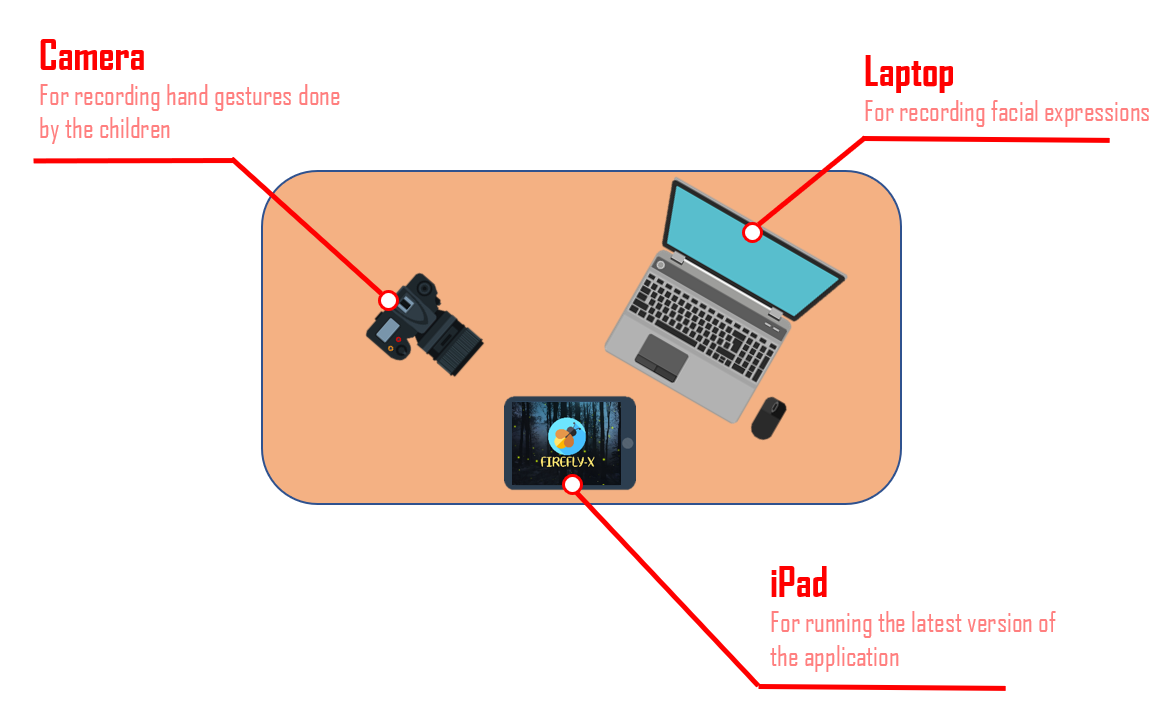
\includegraphics[width=8cm,height=4.5cm]{NewFigures/Test_Setup.png}
    \caption{Iteration 1 and 2 Test Setup}
    \label{fig:test_setup}
\end{figure}

\subsubsection{Participants}
Children that were aged 5-8 either from music schools or had no formal music classes were the ones selected to be the testers of the application. For the children convenience and purposive sampling was used to have different age ranges to see how they will interact with the application. For the first iteration the participants will be n=3.

\subsubsection{Test Protocol}
We did usability tests as the primary method for evaluating our prototype, first the children will first be given a consent form along as the consent from their parents. If they agree with the terms and decided to continue with the testing, they will be given a brief introduction and description of the study along with the objectives and overview. During testing we will encouraged the child to use the think-aloud protocol as this helped us in gathering more inputs on their taught process and the human factors they exhibited in doing their tasks. The testing was conducted where there was little to no audio and visual distractions. We also timed them with the tasks that they did, where we would ask them first if they are ready to begin and then when ready the timer starts until the child's tells the moderator that he/she is done with their task. After the tasks has been done a post-interview session was done and the questions were represented in a liker-style scoring system of 1 - 4, where pictographs that were also color coded were drawn in index cards for the children to better understand these scales and to make this interactive for them: where (1) was represented in the color Yellow which was the highest score where it was really easy, (2) was represented in the color Red denoting it to be moderately easy, (3) was represented in the color Blue denoting it to be moderately hard, and lastly (4) was represented in the color Violet which was the lowest score where the task was really hard for them. Lastly, we rewarded the child after the test by giving them goodies like candies for them feel proud of themselves after completing the usability tests.


%Explain First Iteration
The first iteration of usability testing focused on the users mainly testing the fundamental functionality with only one firefly. We also wanted to gather their feedback on the interface and the design of the firefly. This iteration gave us insights on how we can better improve on the interaction of the user with the system. After developing the application which is 60\% complete, it would be tested with three (3) users. These tasks revolve around the manipulation of the parts/functionality of the firefly. To meet 60\% completeness namely the tail (pattern), wing (repetition), body (tempo), wing (note speed), and the playback engine of one configured firefly. These were the tasks (Table \ref{tasks}) that were asked to be done for the first iteration:

\begin{table}[H]
\centering
\begin{tabular}{|l|l|} 
\hline
Task \# & Task Description                                                                                                                \\ 
\hline
Task 1  & Set the tempo of the firefly by choosing a body type                                                                            \\ 
\hline
Task 2  & \begin{tabular}[c]{@{}l@{}}Set the speed of note of the firefly by choosing a \\setting in the left wing\end{tabular}           \\ 
\hline
Task 3  & \begin{tabular}[c]{@{}l@{}}Set the number of repetitions of the firefly by \\choosing a setting in the right wing\end{tabular}  \\ 
\hline
Task 4  & \begin{tabular}[c]{@{}l@{}}Set the blinking pattern of the firefly by choosing a \\tail type~\end{tabular}                      \\ 
\hline
Task 5  & Tap on the play button to start playing the firefly                                                                             \\ 
\hline
Task 6  & Replace each part of the firefly to modify the sound                                                                            \\ 
\hline
Task 7  & Free play of the environment                                                                                                    \\
\hline
\end{tabular}
\caption{Iteration 1 Tasks}
\label{tasks}
\end{table}
% \begin{enumerate}
%     \item Set the tempo of the firefly by choosing a body type
%     \item Set the speed of note of the firefly by choosing a setting in the left wing
%     \item Set the number of repetitions of the firefly by choosing a setting in the right wing
%     \item Set the blinking pattern of the firefly by choosing a tail type
%     \item Tap on the play button to start playing the firefly
%      \item Replace each part of the firefly to modify the sound
%     \item Free play of the environment
% \end{enumerate}

% %Explain Second Iteration
% The second iteration of usability testing focuses on getting a better understanding of the human factors that children exhibit when doing their tasks. In this iteration we would test the application that is 80\% complete with seven (7) testers. From the seven testers three of them will be retained from the first iteration of testing, meaning we would have four new participants for this iteration. In this iteration we will be implementing the changes based on the comments received from the first iteration of testing. Functionalities such as pitch and release to canvas, in addition with the ability to manipulate the firefly parts will be added to meet the 80\% completeness. The tasks from the first iteration will carry on in the second iteration testing. These are examples of newly added tasks that will be asked to be done for the second iteration:

% \begin{enumerate}
%     \item Tap on the Feed Me Button to start changing the pitch
%     \item Set the pitch of each note by dragging the biscuit on the tray to the staff
%     \item Start replacing the current pitch of a note by clicking Feed Me button again
%     \item Replace the current pitch for one or more notes by dragging the biscuit/s to a higher line in the staff
%     \item Replace the current pitch for one or more notes by dragging the biscuit/s to a lower line in the staff
%     \item Clear the pitch for all notes by selecting the Clear button 
% \end{enumerate}

%Explain the Analysis Protocol

\subsubsection{Data Analysis}

The data from testing came in forms of qualitative and quantitative data. Qualitative data was acquired through video recordings, observations, and interviews. Interviews were done after the testing to validate the observations and also to get feedback on the user experience of the children testing the application. The quantitative data was also acquired in forms of a questionnaire. This form of data was used in evaluating the usability data of the applications different features. This was done for the group to identify the features that have caused inconveniences for the users. For the results of the first iteration of testing, we decided to record their time for completion of each tasks and then later review the videos of our testing in order to adjust their time for completion. This is to see how difficult it was for the users to complete each task given to them. These adjusted times gave us a better understanding on how easy or hard they perceived the tasks were when we asked them the questions during the interview after using the application. This also helped us in discovering the outliers where we initially taught they were as such but after adjusting them they values were not that far off anymore. Using these scores, statistical treatment on the data will then be performed. We computed for the average difficulty of the tasks per children and then made a threshold of the time of their scores comparing the easiest and the hardest score. We then compared the time spent doing the tasks with the difficulty that they answered per participant. The result of this statistical treatment will then be used in deciding on the features that will be retained and what needs to be improved for the version 2 prototype. 




\section{Results and Findings}
\subsection{Formative Results}
Interviewees were gathered by going to music schools and asking if the music teachers were fine being interviewed. We were able to interview 5 music teachers from different music schools. As a prerequisite, they are required to have at least 5 years of experience in teaching music by the time they participate. The demographic of the characteristics of these music teachers are shown in Table \ref{Demographics}.

\begin{table}[H]
\centering
\begin{tabular}{|l|l|} 
\hline
Characteristic  & Total(n=5)    \\ 
\hline
Age (mean \pm   SD [range]) & 39.8 \pm    14.5 [22-57]              \\ 
\hline
\begin{tabular}[c]{@{}l@{}}Sex (n [\%])\\~~~ Male\\~~~ Female\end{tabular}                                                 & \begin{tabular}[c]{@{}l@{}} 4 [80]\\1 [20]\end{tabular}                 \\ 
\hline
Years of Experience (mean \pm   SD [range])                                                                                    & 20.6 \pm    10.4 [7-35]                                                          \\ 
\hline
\begin{tabular}[c]{@{}l@{}}Preferred Teaching Method (n [\%])\\~~~ Suzuki\\~~~ Traditional\end{tabular}                    & \begin{tabular}[c]{@{}l@{}} 3 [60]\\2 [40]\end{tabular}                  \\ 
\hline
\begin{tabular}[c]{@{}l@{}}Specialty (n [\%])\\~~~ Violin\\~~~ Piano\\~~~ Voice\\~~~ Trumpet\end{tabular}                  & \begin{tabular}[c]{@{}l@{}} 2 [40]\\1 [20]\\1 [20]\\1 [20]\end{tabular}  \\ 
\hline
\begin{tabular}[c]{@{}l@{}}Recommended Musical Fundamental \\to Teach (n [\%])\\~~~ Rhythm\\~~~ Pitch \& Rhythm\end{tabular} & \begin{tabular}[c]{@{}l@{}} 3 [60]\\2 [40]\end{tabular}                  \\
\hline
\end{tabular}
\caption{Music Teachers Demographic}
\label{Demographics}
\end{table}

From the interviews of the music teachers, we were able to compile a few key points that will help us identify the needs of children.
\begin{itemize}
    \item It is important to have the children's attention before teaching anything to them.
    \item The child should also be comfortable with the teacher, in addition to this the child must also feel safe and have trust in the teacher. This will help the child in expressing themselves.
    \item There are multiple ways to get the trust of children. Some are: icebreaker, pep talk, talking to them, and asking how their day is going.
    \item The teacher should assess them to know how to teach them.
    \item The teacher should adjust to the child.
    \item Repetition with development is important. Present the same idea differently.
    \item Teacher's passion will pass on the children.
    \item Rhythm must be taught first to children. It is usually done through clapping.
    \item Every session must be interesting and the curiosity of the child must be exploited.
    \item Learning should be step-by-step. Every part must be understood completely before moving on.
    \item Suzuki method teaches discipline to children. By having discipline, the child is able to study more efficiently alone.
    \item Traditional Method is just teaching the topic to the child. It is more of a by-the-book method, and usually instructional.
\end{itemize}

% Based on our interviews with the music teachers, we were able to hypothesize some features needed by children. These hypotheses were then clarified with them and verified. After these, it was then translated into features for the mid-fidelity prototype.

% \begin{table}[H]
% \begin{tabular}{|p{8cm}|}
% \hline
% \begin{tabular}[c]{@{}l@{}}\textbf{H:} Children would want to edit existing fireflies and explore \\other options or settings. \\ \textbf{C:} Asked the music teacher if the child will \\edit existing fireflies.\\ \textbf{V:} Verified that the child would want to have the option \\to edit fireflies. This will allow the child to explore\\other combinations.\\ \textbf{T:} Added feature that allowed fireflies to be edited \\before released.\end{tabular} \\ \hline
% \begin{tabular}[c]{@{}l@{}}\textbf{H:} The child would want to replay previous tracks.\\ \textbf{C:} Asked the teacher if the child will replay previous tracks.\\ \textbf{V:} Verified that the child will want to replay previous tracks \\and listen again to the track. This will let the child to  have a \\clearer understanding on how the configurations affected \\the sound produced.\\ \textbf{T:} Added a feature that allowed replaying of previous tracks.\end{tabular} \\ \hline
% \begin{tabular}[c]{@{}l@{}}\textbf{H:} The child would want to save and load workspace.\\\textbf{C:} Asked the teacher if the child would want to save \\the existing workspace or load an existing workspace.\\ \textbf{V:} Verified that the child would want to save the existing \\workspace to allow them to exit the workspace anytime \\or load a workspace anytime. This will allow the child to have\\the freedom of continuing whenever they want to.\\ \textbf{T:} Added feature that allowed the saving of existing \\workspace, and loading of an existing workspace. \end{tabular} \\ \hline
% \begin{tabular}[c]{@{}l@{}}\textbf{H:} The child would want to reset the workspace and delete all \\configurations of the fireflies.\\ \textbf{C:} Asked the teacher if the child would want to reset the\\workspace.\\ \textbf{V:} Verified that the child would want to reset the workspace \\and reset all the configurations of the fireflies. \\This will allow the child to quickly get rid of all \\the configurations and start from scratch.\\ \textbf{T:} Added feature that allowed resetting the workspace and \\delete all the configurations of the fireflies.\end{tabular} \\ \hline
% \end{tabular}
% \caption{Basic Feature Translations. H = Hypothesis, C = Clarification,  V =Verification, T = Translation.}
% \label{table:BasicFeatureTranslations}
% \end{table}

\subsection{Music Language}
To help us better understand the music sheets from the Book 1 of the Suzuki teaching method, we decided to convert the sheets to a language we can easily understand and represent on code. See Table \ref{patterns} for reference to the most common patterns from the Suzuki book 1 converted language. This will mainly be used for the representation for the first iteration since at this iteration it only covers rhythm. To make the app easier to use, a set of rules for the music composition has been used. The firefly will only be using a maximum of 6 measures per rhythm. Each measure is equal to 1 pattern. The speed of the notes and rests that will be supported by the application will only be the whole, half, quarter, and eighth note.

For the representation in the table, 1 is for the clap and the 0 is for the rest. An example as seen from the table is "1Rest" - the number 1 coefficient represents the number of instances of the rest. A change in pattern from rest to tap is separated by a dash. 

\begin{table}[H]
\begin{tabular}{|l|l|l|}
\hline
Pattern & Pattern Name            & Note Count                \\ \hline
0       & 1Rest                   & {[}Wr-23{]}               \\ \hline
1010    & 1Clap-1Rest-1Clap-1Rest & {[}QQrQQr - 39{]}         \\ \hline
1111    & 4Clap                   & {[}QQQQ - 21, EEQH - 1{]} \\ \hline
10110   & 1Clap-1Rest-2Clap-1Rest & {[}QQrEEQr - 26{]}        \\ \hline
\end{tabular}
\caption{Most Common Patterns Seen on Suzuki Book 1}
\label{patterns}
\end{table}

\subsection{Prototype Features and Screen Flow}
\begin{figure}[H]
    \centering
    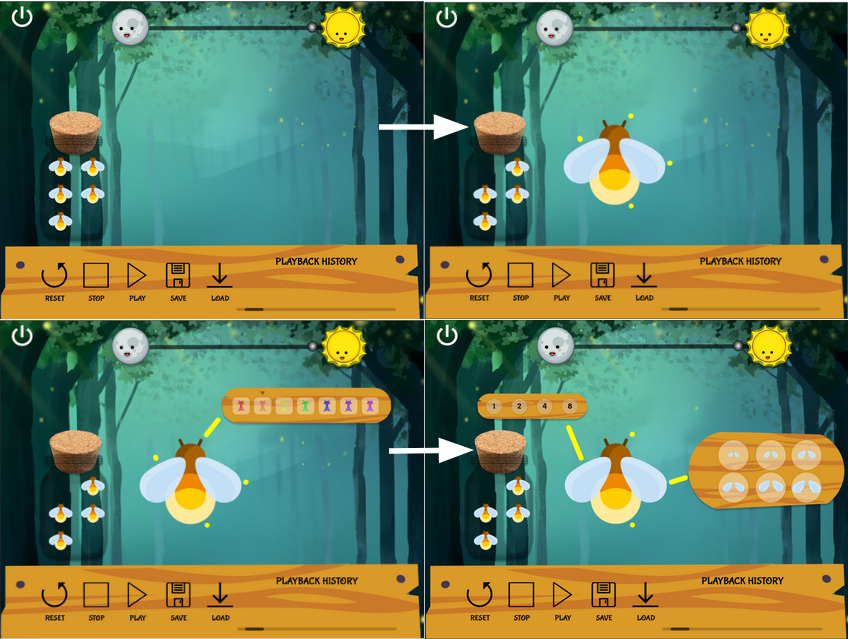
\includegraphics[width=8cm]{NewFigures/RESTCON1.png}
    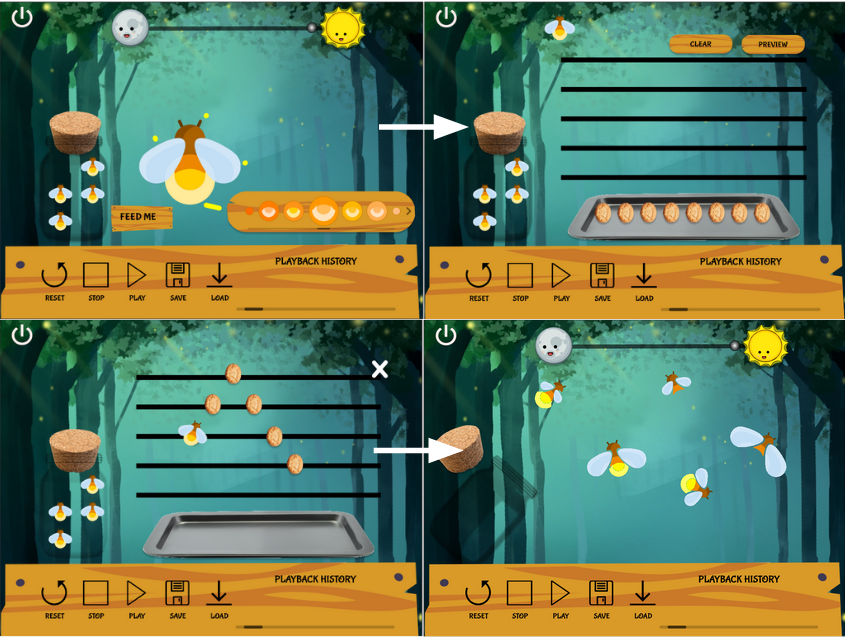
\includegraphics[width=8cm]{NewFigures/RESTCON2.png}
    \caption{Screen Flow}
    \label{fig:Screenflow1}
\end{figure}
% \subsubsection{Choose a Firefly to Edit}
% The user taps a firefly in the jar to start editing the parts.

% \subsubsection{Set Tempo}
% The user taps the body to choose the tempo of the firefly.

% \subsubsection{Set Note length}
% The user taps the left wing to choose the first note of the firefly.

% \subsubsection{Set Number of Repetition}
% The user taps the right wing to choose the number of repetitions

% \subsubsection{Set Pattern}
% The user taps the Tail to choose the pattern of the beats and rests.

% \subsubsection{Set Pitch}
% The user taps the the feed me button to set the pitch of the notes using cookies.

% \subsubsection{Release All Fireflies Playback}
% This feature allows the user to preview what happens when the user is done configuring all fireflies, and has released them from the jar to start playback.
\begin{table}[H]
\label{screenflows}
\caption{Screen Flows}
\begin{tabular}{|l|l|}
\hline
Screen                                                                    & Action                                                                                                                                                                                                       \\ \hline
\begin{tabular}[c]{@{}l@{}}Choose a Firefly\\  to Edit\end{tabular}       & \begin{tabular}[c]{@{}l@{}}The user taps a firefly in the jar to start \\ editing the parts.\end{tabular}                                                                                                    \\ \hline
Set Tempo                                                                 & \begin{tabular}[c]{@{}l@{}}The user taps the body to choose the tempo \\ of the firefly.\end{tabular}                                                                                                        \\ \hline
Set Note length                                                           & \begin{tabular}[c]{@{}l@{}}The user taps the left wing to choose the \\ first note of the firefly.\end{tabular}                                                                                              \\ \hline
\begin{tabular}[c]{@{}l@{}}Set Number of \\ Repetition\end{tabular}       & \begin{tabular}[c]{@{}l@{}}The user taps the right wing to choose the \\ number of repetitions\end{tabular}                                                                                                  \\ \hline
Set Pattern                                                               & \begin{tabular}[c]{@{}l@{}}The user taps the Tail to choose the \\ pattern of the beats and rests.\end{tabular}                                                                                              \\ \hline
Set Pitch                                                                 & \begin{tabular}[c]{@{}l@{}}The user taps the the feed me button to set \\ the pitch of the notes using cookies.\end{tabular}                                                                                 \\ \hline
\begin{tabular}[c]{@{}l@{}}Release All \\ Fireflies Playback\end{tabular} & \begin{tabular}[c]{@{}l@{}}This feature allows the user to preview what \\ happens when the user is done configuring all\\  fireflies, and has released them from the jar \\ to start playback.\end{tabular} \\ \hline
\end{tabular}
\end{table}

\subsection{Iteration 1 Features}

\subsubsection{Set Tempo}
The body section of the firefly model can be tapped to show the popup settings. In the popup settings of the body section, the user is able to choose the tempo of the taps that the firefly will play. Each unique color of the body has an equivalent tempo. 

\subsubsection{Set Note length}
The left wing section of the firefly model can be tapped to show the popup settings. In the popup settings of the left wing section, the user is able to choose the speed of the  beat being played by pressing 1, 2, 4, or 8 which represents the whole note/rest, half note/rest, quarter note/rest, eighth note/rest, respectively based on the setting of the lever.

\subsubsection{Set Note or Rest}
In the left wing section of the firefly model there is a lever above the popup settings. A tap gesture was implemented for the lever. In the lever, the user is able to choose if the first beat is either a note or a rest.

\subsubsection{Set Number of Repetition}
The right wing section of the firefly model can be tapped to show the popup settings. In the popup settings of the right wing section, The size of the wing will represent the number of repetitions. The minimum size is 1 and the maximum size is 6.

\subsubsection{Set Pattern}
The tail section of the firefly model can be tapped to show the popup settings. On the right side, the user is able to change the rest pattern of the note being played based on the first beat that was selected by the user. The tail lights will be blinking patterns and pattern can be previewed in popup settings, the light will be based from the chosen color in the body.



\subsection{Iteration 1 Testing Results}

% Table \ref{tab:iter1results} shows the overview of the results from the acquired data from the feedback form from Iteration 1, while Table \ref{tab:iter2results} shows the results from Iteration 2. As mentioned, the feedback forms from those iterations differed, so the results and treatment of the data will be discussed separately in the following subsections.

\begin{table}[H]
\centering
\begin{tabular}{|l|l|l|l|l|l|l|} 
\hline
   & Age & Years & Sex & Hand & Instrument                                                          & Technique  \\ 
\hline
P1 & 8   & 1     & M   & R    & Drums                                                               & T          \\ 
\hline
P2 & 7   & 1     & F   & L    & \begin{tabular}[c]{@{}l@{}}Piano and \\Drums \end{tabular}          & T          \\ 
\hline
P3 & 5   & 1     & M   & R    & \begin{tabular}[c]{@{}l@{}}Piano, Guitar, \\and Drums \end{tabular} & T          \\
\hline
\end{tabular}
\caption{Participant Demographic. T - Traditional, S - Suzuki}
\label{participant}
\end{table}


We processed the timestamps in order to normalize these values. This is important so we can properly understand the actual time it took them to finish the task, this can be seen in Figures \ref{fig:P1Timing}, \ref{fig:P2Timing}, and \ref{fig:P3Timing}. We then observed that due to other circumstances during the testing like the long duration and fatigue from school, in answering the questions the children sometimes mistook the scales in grading for the difficulty of the tasks. In some tasks they graded it much easier or harder than what we observed as when we double checked and asked them to name the functionality of a specific part, they were mixing up some of the functionality yet still for example give a score of (1) where they fully remembered it. Due to this their initial scores were then cross referenced to the task they were given and if we observed that there was a big difference in the answer and our observation an adjustment of  + 1 or - 1 was changed in the scores to balance these out. 

The red bar indicates the level of difficulty that the user has chosen for the task. The blue bar indicates the time for their time of completion for the task. To enhance the visualization we scaled the difficulty of 1-4 by multiplying it by 5 and divided their time by 5 so their correlation can be seen more in the graphs.

\begin{figure}[H]
    \centering
    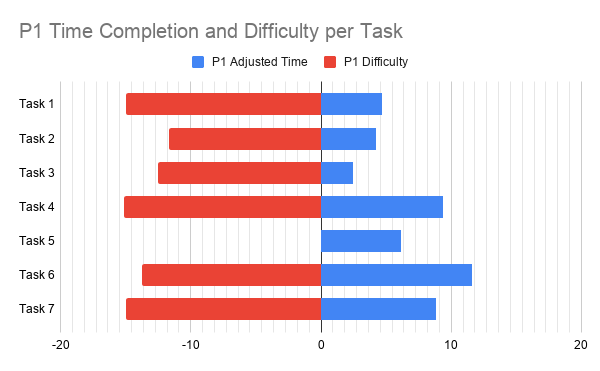
\includegraphics[width=8cm]{NewFigures/P1.png}
    \caption{Time for Completion and Difficulty of Tasks for Person 1}
    \label{fig:P1Timing}
\end{figure}
 P1 (8, M, Drums) believes that task 4, which was the tail, was most likely not intuitive for him to change because it took him a longer time and he rated it as a higher difficulty compared to playing with the other body parts. Task 6 and 7 took a long time because it was mostly playing around with the application.
 
\begin{figure}[H]
    \centering
    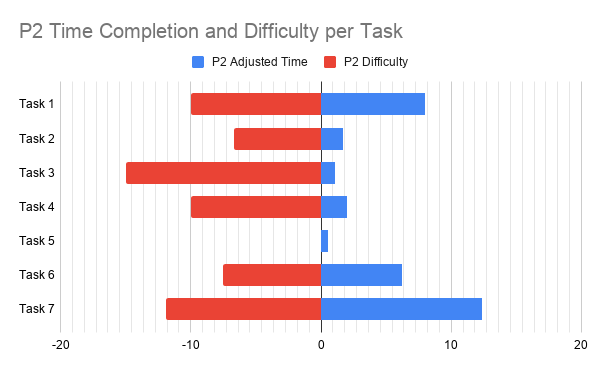
\includegraphics[width=8cm]{NewFigures/P2.png}
    \caption{Time for Completion and Difficulty of Tasks for Person 2}
    \label{fig:P2Timing}
\end{figure}
P2 (7, F, Piano) believes that task 2, which is the body, was most likely not intuitive because it took her a long time to complete. It can also be seen also that she did not grade the difficulty as high as person 1 because she has more experience in music.

\begin{figure}[H]
    \centering
    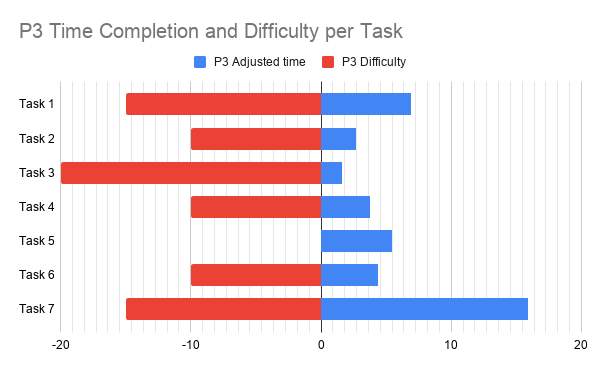
\includegraphics[width=8cm]{NewFigures/P3.png}
    \caption{Time for Completion and Difficulty of Tasks for Person 3}
    \label{fig:P3Timing}
\end{figure}
P3 (5, M, Guitar) similar to P2 took a lot of time in performing task 1 which supports that it most likely not intuitive.


% Based on observations and comments from the Focus Group Discussions, participants appreciated and had a more positive response to the louder and faster songs. All participants agreed that the inclusion of speakers for haptic feedback and colors would improve their experience, as such this was considered for the Iteration 2 experiments. The participants were easily bored due to the grayscale color scheme of the prototype. The participants provided more recommendations such as (1) adding the lyrics as captions (2) visuals of the singer singing the song and (3) adding more visual elements.

% Based on the data in Figure \ref{tab:iter1results}, we computed for the correlation coefficients of BPM with average score and BPM with standard deviation, which can be seen in Table \ref{tab:correlations}. Based on these statistical figures, BPM and average score, as well as standard deviation have no correlation.
% %The computed correlation coefficient for BPM and average score is 0.1294, which is interpreted as little positive correlation. The computed correlation coefficient for BPM and standard deviation is 0.1145, which is also interpreted as little correlation.

% Despite the explicit statements from the participants that they appreciated the louder and faster songs, analysis of the statistical results show that their scores were not consistent. Faster and louder songs did not necessarily have the higher ratings. This may be attributed to mismatches regarding visual impact. The songs may not have had their musical features represented consistently and fairly enough for them to appreciate the experience.


\begin{figure}[H]
    \centering
    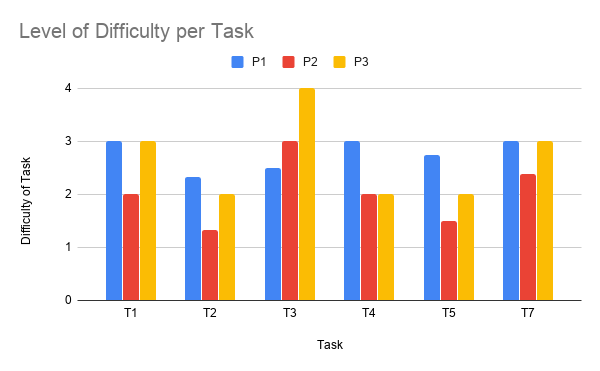
\includegraphics[width=8cm]{NewFigures/DifficultyTask.png}
    \caption{Difficulty of Tasks for each User}
    \label{fig:DifficultyofTask}
\end{figure}
\begin{figure}[H]
    \centering
    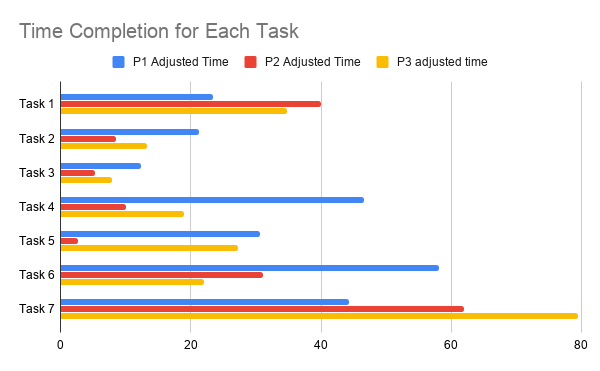
\includegraphics[width=8cm]{NewFigures/AllTime.png}
    \caption{Time Completion of Tasks for each User}
    \label{fig:TimeofTask}
\end{figure}

\subsection{Participant Insights}

\begin{figure}[H]
    \centering
    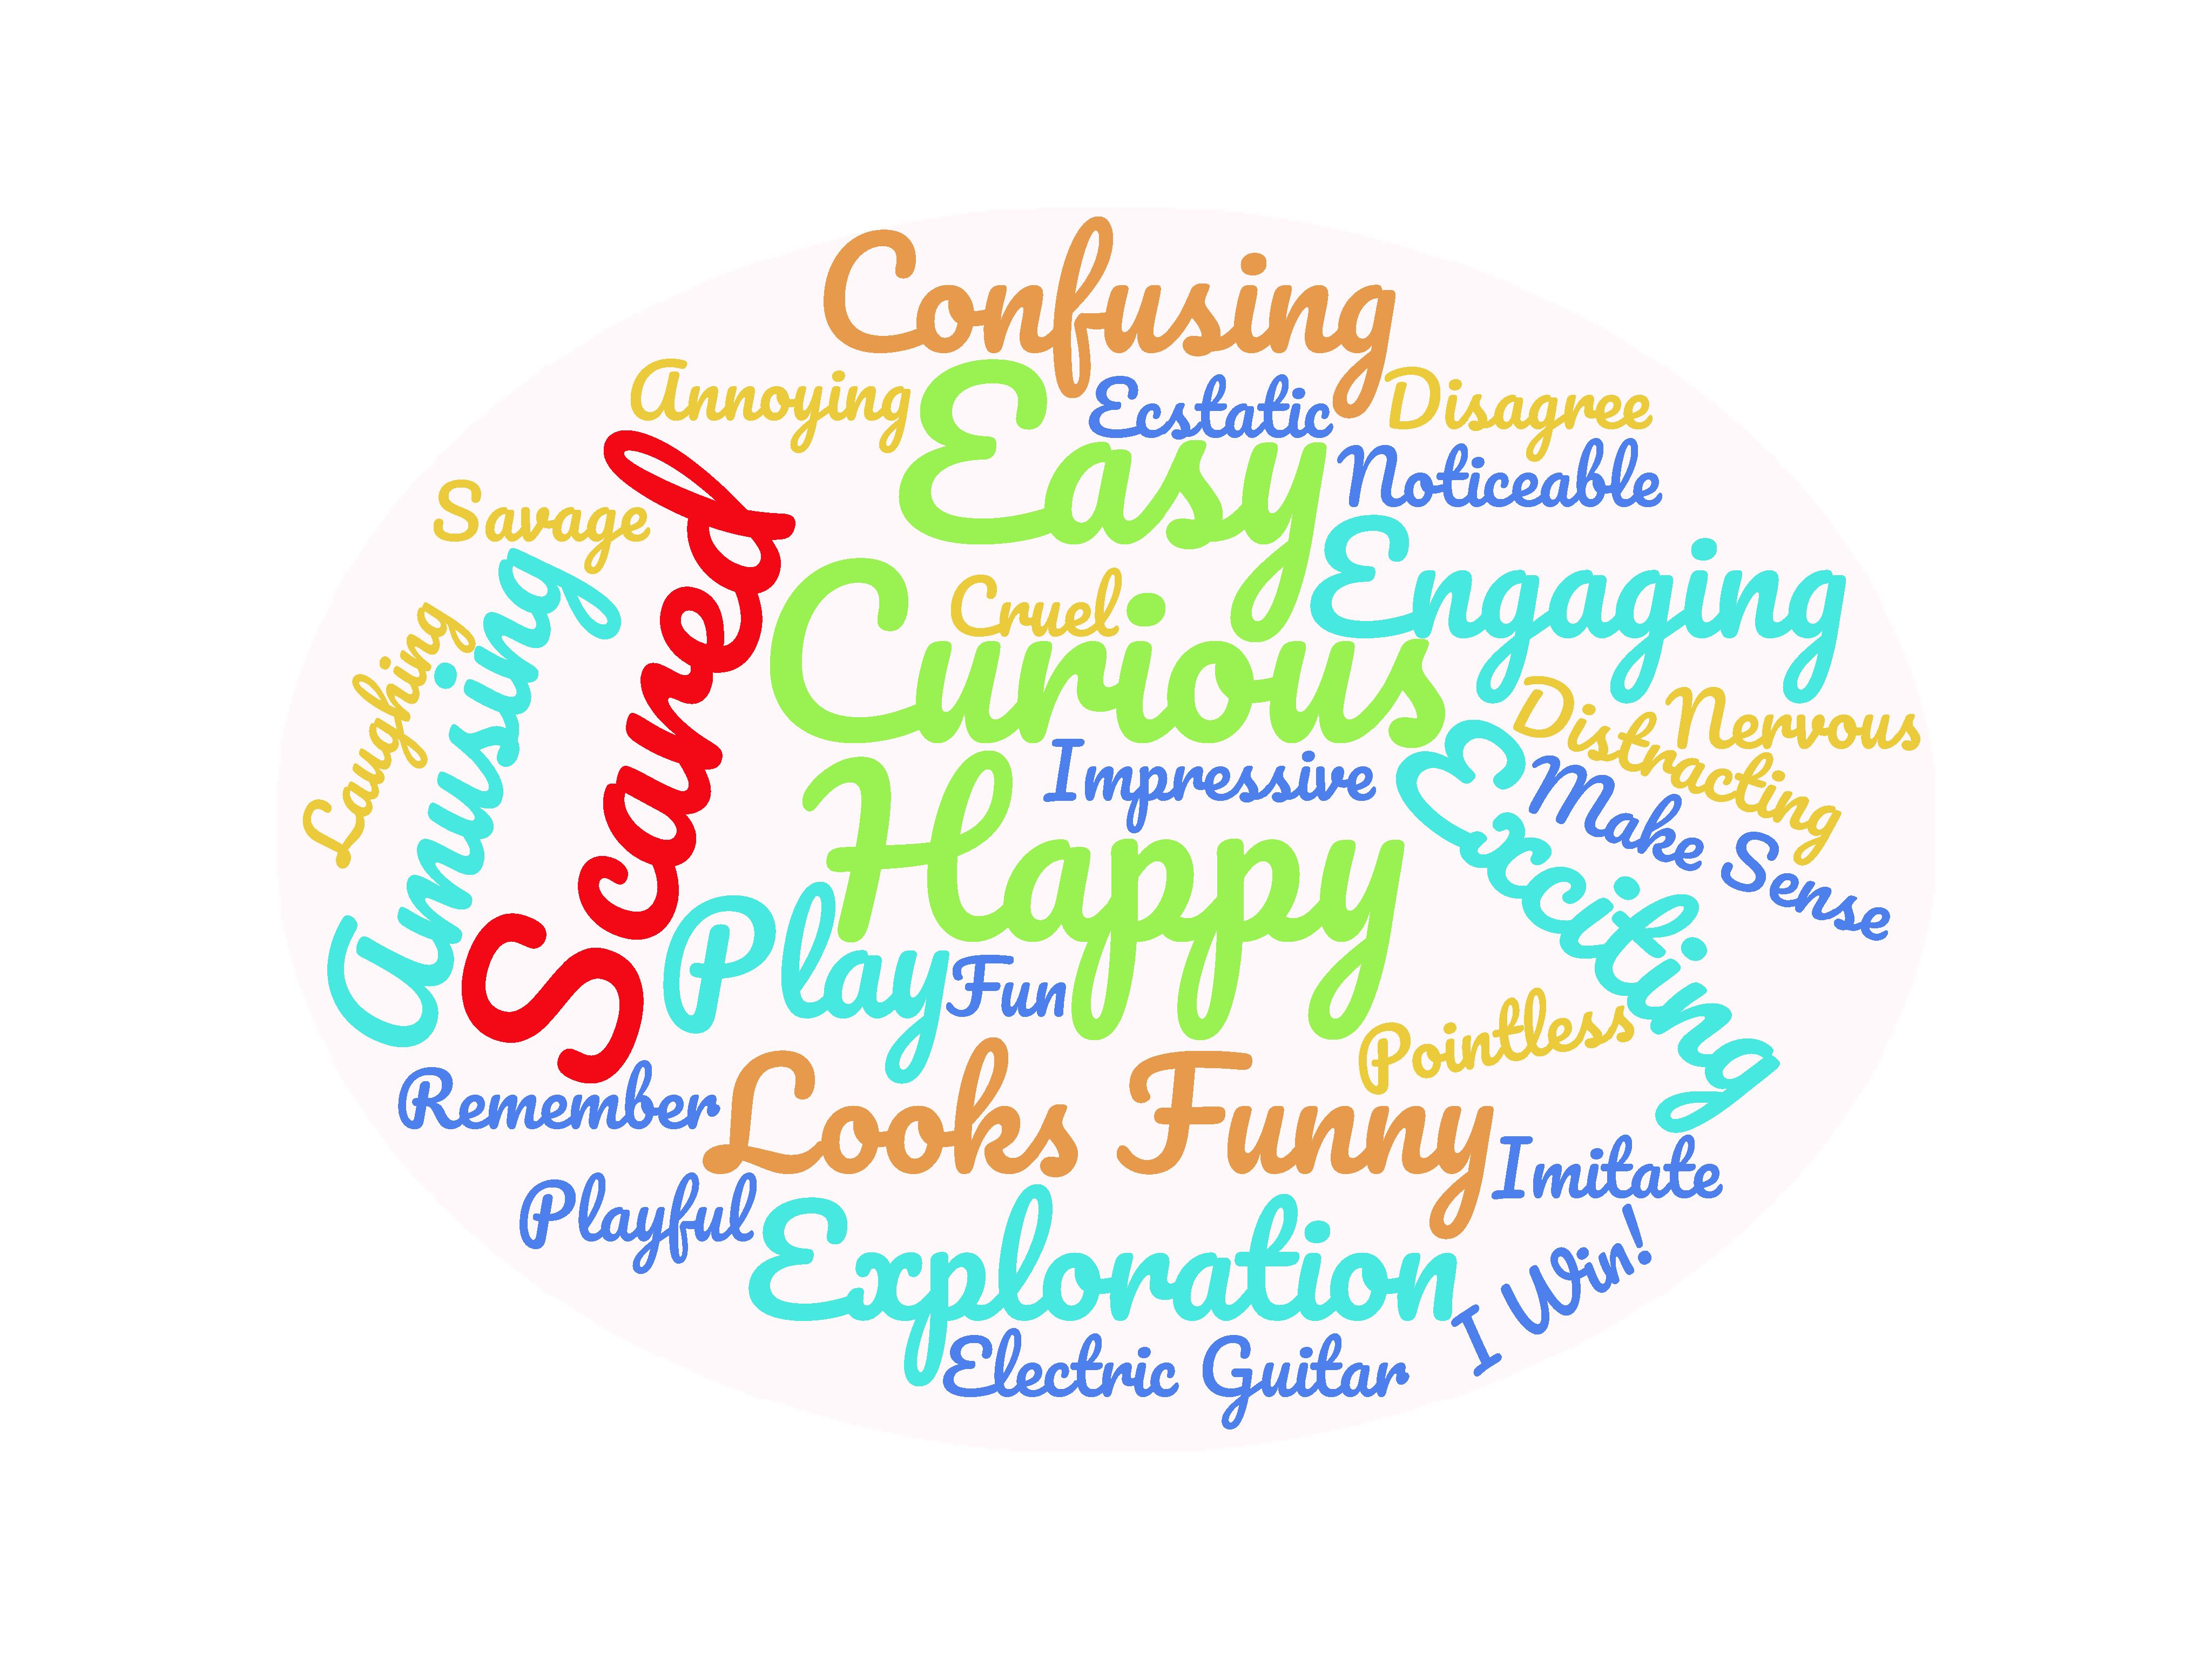
\includegraphics[width=9.5cm]{NewFigures/wordcloud.jpg}
    \caption{Word Cloud of Positive and Negative Comments}
    \label{fig:wordcloud}
\end{figure}

% \begin{figure}[H]
%     \centering
%     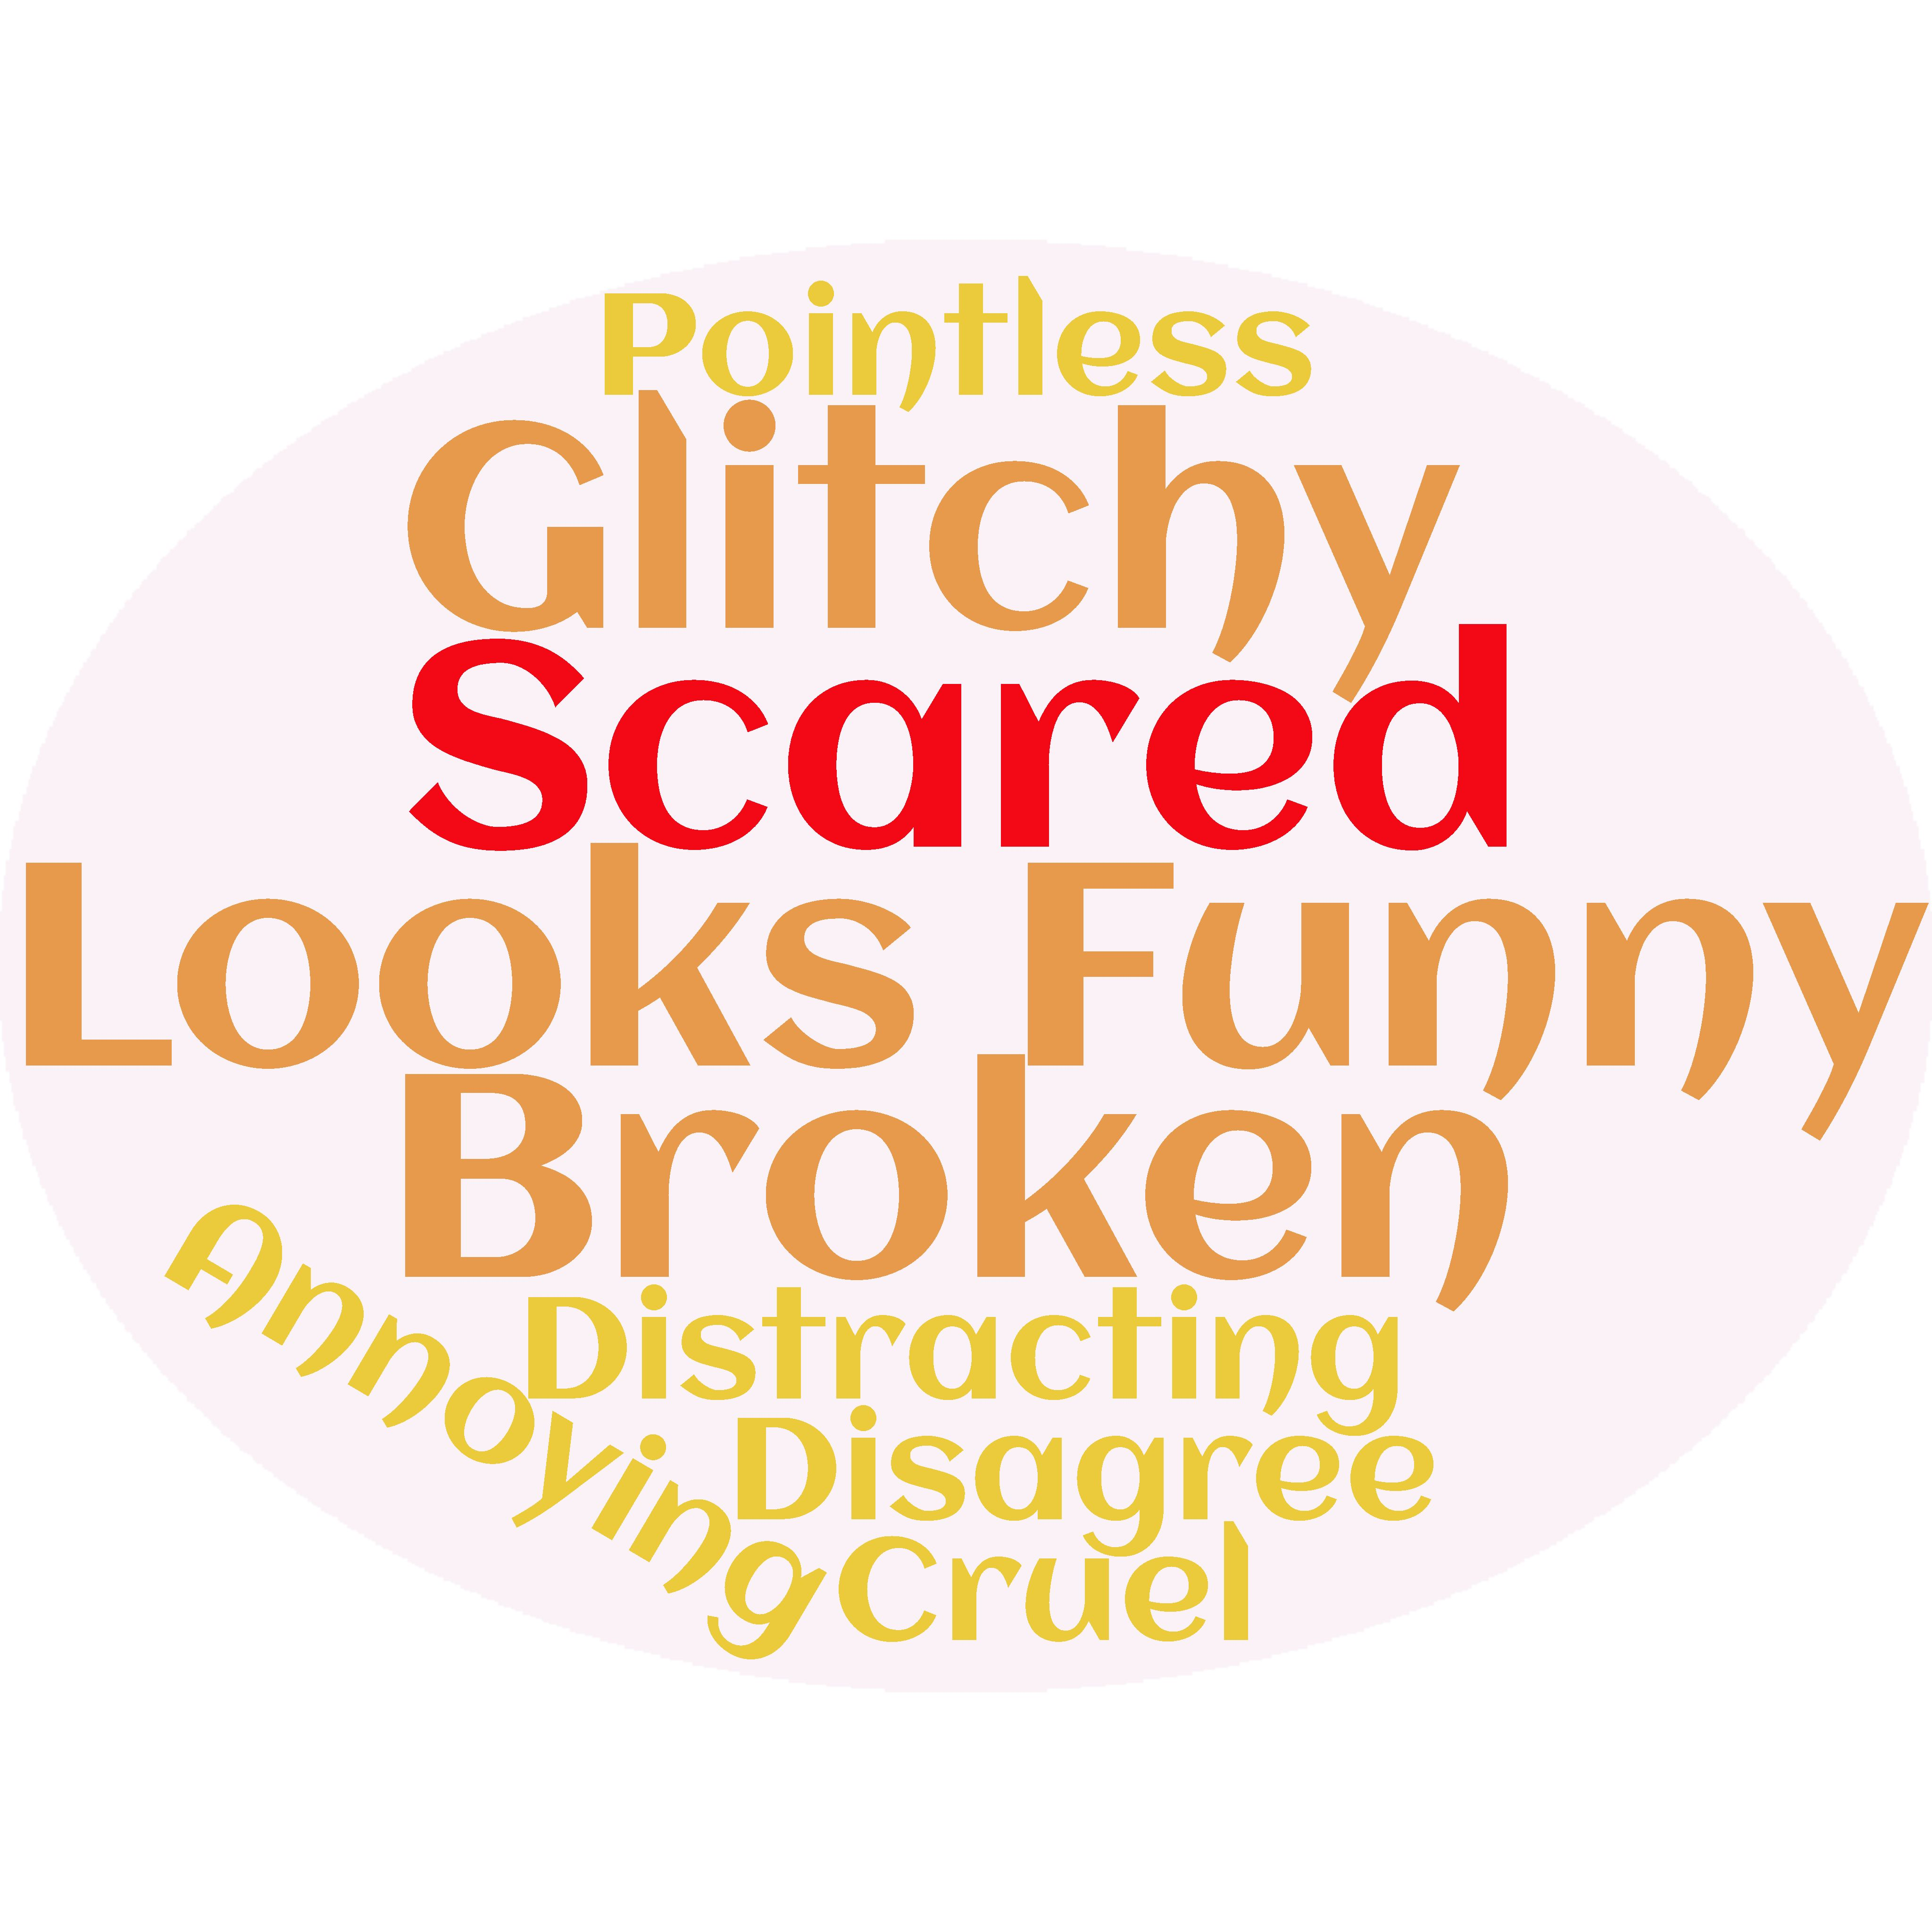
\includegraphics[width=8cm]{NewFigures/negativeWordcloud.jpg}
%     \caption{Word Cloud of Negative Comments}
%     \label{fig:negative}
% \end{figure}


\section{Discussion}

It can be seen clearer in Section 4.5 that majority of them took longer in playing with the body part, which is task 1. And upon further observation one of the underlying reasons could be that they tend to miss the hotspot for pressing the body part.  We also noticed that most of them would pick their favorite color for the body part, which they enjoyed. It can also be seen that Task 3 which is changing the size of the wings for repetition took them the fastest time to complete

Based on our user testing for iteration one, as seen in Figure \ref{fig:DifficultyofTask}, task two, which was to change the speed of the first note using the left wing, took the shortest time to complete and had the lowest difficulty for the users. However, in task two only two out of three users noticed the lever for changing the note to rest or beat. Then task 3, which was to change the number of repetitions by tapping the right wing, took the longest time and had the highest difficulty for the users. We also observed that all participants use their dominant hand most of the time when using the application as P1 and P3 were both right handed as P2 was the only one that was left handed. During the interview some had a hard time remembering which part of the firefly changed each property when they were asked which part did what. The one with most music experience mentioned that the app didn't help much in retaining her music lessons, and then suggested that we utilize a music staff. We observed their behavior when using the application and we noticed that they were eager to explore features that they think is clickable even when the tasks were not yet given to them. We also noticed that in features like the lever, they would use a flick gesture imitating how it is usually used instead of the tap gesture that we set it to be. 

 As seen in Figure \ref{fig:wordcloud} during testing while they were doing their tasks we took note of their comments and interpreted them in a general way or in terms of a feature that they commented on. The positive comments were represented using cool colors like blue and green, while negative comments were represented with warm colors like red and orange. For the positive comments we observed that aside from us noticing their curiosity in using the application, they themselves say that they are curious when doing their tasks. We can also see that they have comments about being playful and having fun while using the application. In terms of the interface, comments like "Make Sense" and "Engaging" indicated to us that there are features that they like and that some parts of the interface is good for them. For the negative comments, one comment that stood out to us was P3 mentioned that the animations of the firefly was "glitchy", this comment made us improve the assets for the animation for the next animation. The other negative comments like "Looks Funny" and "Distracting" indicated to us that there were some features that they wanted us to change in the interface. Lastly, even if the purpose of the sandbox environment was for the users to play without breaking anything, P3 still said he was "Scared" multiple times to ruin the firefly and we think that this has to do with his young age and also for us to put information on the screen so that the children will not be discouraged to play with the firefly.
 

% \subsection{Iteration 2 Features}

% \subsubsection{Set Pitch}
% The mode is only accessible upon tapping the feed me button. The feed me button can be accessed during the tail pop settings once the user has already selected a pattern. There will be a staff where the candies may be placed. The candies will be representing the notes. The number of candies will depend on the number of claps in the chosen pattern. A drag gesture was implemented so that the candies can be set in a specific pitch that the child would want. The candies have a different design based on the duration of the notes and rests. The placement of the notes will also be determining the flight pattern of the firefly model.

% \subsubsection{One Firefly Playback}
% This feature allows the user to preview the configured firefly after setting the pitch. The user will be able to hear the music he has produced using the parts of the firefly.
% \begin{figure}[H]
% 	\centering
% 	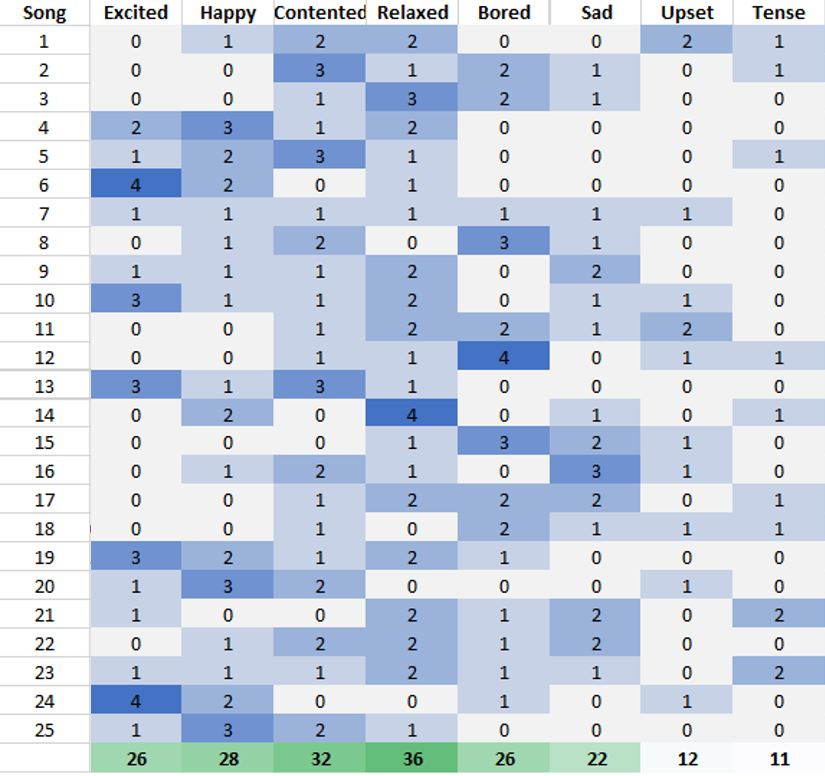
\includegraphics[width=1\columnwidth]{figures/iter2results.JPG}
%     \caption{Iteration 2 Feedback Form Results}
%     \label{fig:iter2results}
% \end{figure}

% \begin{table*}[t]
%   \centering
%   \caption{Iteration 2 Feedback Form Results}~\label{tab:iter2results}
%   \addtolength{\tabcolsep}{2pt} 
%   \begin{tabular}{P{2.5cm}|P{1cm}|P{0.9cm}|P{1cm}|P{1cm}|P{0.9cm}|P{0.9cm}|P{0.9cm}|P{0.9cm}|>{\bfseries}P{2.5cm}}
%   	\toprule
%     \rule{0pt}{8pt}Song & Excited & Happy & Content & Relaxed & Bored & Sad & Upset & Tense & Total per Song\\[2pt]
%     \toprule
%     1 & 0 & 1 & 2 & 2 & 0 & 0 & 2 & 1 & 8 \\ \hline
%     2 & 0 & 0 & 3 & 1 & 2 & 1 & 0 & 1 & 8 \\ \hline
%     3 & 0 & 0 & 1 & 3 & 2 & 1 & 0 & 0 & 7 \\ \hline
%     4 & 2 & 3 & 1 & 2 & 0 & 0 & 0 & 0 & 8 \\ \hline
%     5 & 1 & 2 & 3 & 1 & 0 & 0 & 0 & 1 & 8 \\ \hline
%     6 & 4 & 2 & 0 & 1 & 0 & 0 & 0 & 0 & 7 \\ \hline
%     7 & 1 & 1 & 1 & 1 & 1 & 1 & 1 & 0 & 7 \\ \hline
%     8 & 0 & 1 & 2 & 0 & 3 & 1 & 0 & 0 & 7 \\ \hline
%     9 & 1 & 1 & 1 & 2 & 0 & 2 & 0 & 0 & 7 \\ \hline
%     10 & 3 & 1 & 1 & 2 & 0 & 1 & 1 & 0 & 9 \\ \hline
%     11 & 0 & 0 & 1 & 2 & 2 & 1 & 2 & 0 & 8 \\ \hline
%     12 & 0 & 0 & 1 & 1 & 4 & 0 & 1 & 1 & 8 \\ \hline
%     13 & 3 & 1 & 3 & 1 & 0 & 0 & 0 & 0 & 8 \\ \hline
%     14 & 0 & 2 & 0 & 4 & 0 & 1 & 0 & 1 & 8 \\ \hline
%     15 & 0 & 0 & 0 & 1 & 3 & 2 & 1 & 0 & 7 \\ \hline
%     16 & 0 & 1 & 2 & 1 & 0 & 3 & 1 & 0 & 8 \\ \hline
%     17 & 0 & 0 & 1 & 2 & 2 & 2 & 0 & 1 & 8 \\ \hline
%     18 & 0 & 0 & 1 & 0 & 2 & 1 & 1 & 1 & 6 \\ \hline
%     19 & 3 & 2 & 1 & 2 & 1 & 0 & 0 & 0 & 9 \\ \hline
%     20 & 1 & 3 & 2 & 0 & 0 & 0 & 1 & 0 & 7 \\ \hline
%     21 & 1 & 0 & 0 & 2 & 1 & 2 & 0 & 2 & 8 \\ \hline
%     22 & 0 & 1 & 2 & 2 & 1 & 2 & 0 & 0 & 8 \\ \hline
%     23 & 1 & 1 & 1 & 2 & 1 & 1 & 0 & 2 & 9 \\ \hline
%     24 & 4 & 2 & 0 & 0 & 1 & 0 & 1 & 0 & 8 \\ \hline
%     25 & 1 & 3 & 2 & 1 & 0 & 0 & 0 & 0 & 7 \\ \hline
    
%     \textbf{Total per Affect} & \textbf{26} & \textbf{26} & \textbf{32} & \textbf{36} & \textbf{26} & \textbf{22} & \textbf{12} & \textbf{11} & \textbf{193} \\
%     \bottomrule
%   \end{tabular}
%   \addtolength{\tabcolsep}{-2pt} 
% \end{table*}

% Based on observations and comments from the Focus Group Discussion, the participants welcomed the use of more colors and shapes. One thing the researchers also noticed was that the younger participants appreciated the visuals more than the haptic feedback from the speakers, while the opposite was true for the older participants. This may have been because the balloons for feeling the vibrations were given only to the older participants. Just as with the first iteration, the participants also suggested to include song lyrics. A new suggestion was to show wavelength visualization, which they felt would help them better understand the dynamics of the music being played. For future iteration testing, it has also been suggested that listeners rest in between songs. % Should we remove statement on younger vs older participants?

% The checkmarks from the feedback forms were tallied and tabulated. Table \ref{tab:iter2results} shows the number of participants that felt a certain affect per song. Based on the data from Table \ref{tab:iter2results}, we computed the correlation coefficients of BPM with the different affects, which can be seen in Table \ref{tab:correlations}. Although there were some noticeable correlations between the speed of the song (BPM) and the affects felt, such as with happiness and upsetness, little to no correlations were observed in the other affects. Just as in the previous experiment, the visual impact may have also been a factor, but was again not included in this quantitative analysis since it may not be quanitified. The updated prototype in this iteration was generally more welcomed than the previous one. More attention was given to giving the musical features more justice in this iteration, which allowed for the main features of the visualizer to be laid down. The next step was to refine the visualizations and make them more aesthetically pleasing.

%For the high-valence and high-arousal affects, BPM vs Excitement has a computed coefficient of 0.0098, which is almost no correlation, while BPM vs Happiness has a computed coefficient of 0.4397, which is some positive correlation. For the high-valence and low-arousal affects, BPM vs Contentment has a computed coefficient of 0.2918, which is little positive correlation, while BPM vs Relaxment has a computed coefficient of -0.2126, which is little negative correlation. For the low-valence and low-arousal affects, BPM vs Boredom has a computed coefficient of -0.183, which is little negative correlation, while BPM vs Sadness has a computed coefficient of -0.1509, which is little negative correlation. For low-valence and high-arousal affects, BPM vs Upsetness has a computed coefficient of -0.3310, which is some negative correlation, while BPM vs Tension has a computed coefficient of -0.1500, which is little negative correlation.

%\subsection{Iteration 3}

% Iteration 3 results

\section{Conclusion \& Future Work}
% Conclusion

% This study provides a framework for a visualization system to augment the musical experience of the DHH. To achieve this, we had to perform needfinding and conceptualization which included interviews with members of the DHH community and interpreters, as well as review of related literature in order to conceptualize the approach to building the tool. As the study is still ongoing, some features are not yet fully implemented. However, qualitative feedback from members of the DHH community suggest that the tool may be helpful towards their musical experience as a whole. Regarding the four (4) contributions attempted to be made by this research, we can conclude at this point that (1) the interaction designed does improve how the DHH experience music, (2) the use of a movie roll visualization scheme is effective for the purpose of augmenting musical experience, and (3) the developed framework to process and understand music samples is capable of generating appropriate visualizations. However, the generated visuals are still to be improved upon and made more appropriate. As this study is still ongoing, (4) we can not yet say whether we have successfully and completely evaluated whether these ultimately augment the music experiences of the DHH.

In this study, we were able to understand how children were taught music by their music teachers. The findings can be seen in Section 3.1 and 3.2, where we were able to get their insights and converted them into artifacts that guided us in developing the application. We were then able to design the interaction for the gestures that were integrated to the features of the application as seen in Section 4.3 and 4.3. Lastly, we were able to observe early findings on the time it took them to complete the task vs their perceived difficulty, this can be seen in the results found in Section 4.5 and the discussion in Section 5, but this can be subject to more testing.

% Future work
For future work, we intend to perform more testing of the application, where the data gathered from the first iteration will be considered to improve the features of the application and also introduce new features as well. The authors also believe that there is a need to perform these tests with more participants to have a more diverse understanding on the learning of different children. Since the current application only provides learning for an individual child, a collaboration feature can be worked on so that children can help their learning as a group by either configuring the fireflies together or sharing their firefly configurations while using the application.


% Future work for this study includes a third iteration, where the data and feedback gathered from the first two iterations will be considered when making improvements to the system prototype and the experiment setup. Because of the suggestions from both previous iterations, for the third and succeeding iterations, we plan to (1) include showing lyrics as captions, we will include said feature in the prototype and (2) give participants time to rest in between songs.


% \begin{acks}
% The authors would like to thank Mr. Ralph Gonzalez for his expertise in music, and helping us understand its relation to emotion.

% The authors would also like to thank the De La Salle-College of Saint Benilde School of Deaf Education and Applied Studies (DLS-CSB SDEAS) for sharing their knowledge on the DHH Community and coordinating with members of the DHH Community in order to provide participants for this study.

% Finally, the authors thank the testing participants themselves for their valuable time and feedback.
% \end{acks}